\ylDisplay{Oktaeeder} % Ülesande nimi
{Jaan Kalda} % Autor
{lahtine} % Voor
{2016} % Aasta
{G 8} % Ülesande nr.
{8} % Raskustase
{
% Teema: Elektriahelad
\ifStatement
Juuresolev skeem kujutab traadist oktaeedrit, iga traadi juurde on kirjutatud selle takistus oomides. 
Ampermeetreid ühendavad traadid on tühiselt väikese takistusega.
Leidke ampermeetrite näidud.

\begin{center}
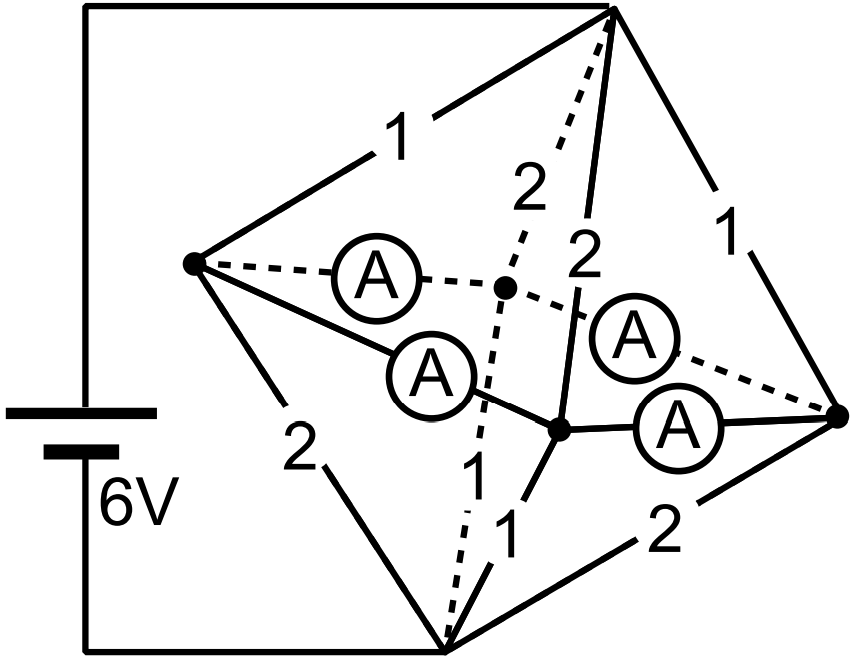
\includegraphics[width=0.5\textwidth]{2016-lahg-08-ampermeeterjoonis.png}
\end{center}
\fi


\ifHint
Et ampermeetrite sisetakistus on \num{0}, siis võime need lühistada: kõigis nendes tippudes, kuhu viivad ampermeetrid, on potentsiaalid võrdsed. Sümmeetria tõttu peab see 
potentsiaal jääma täpselt patareiklemmide potentsiaalide vahepeale, seega on igale takistile rakendatud pinge
$\SI 3V$.
\fi


\ifSolution
Et ampermeetrite sisetakistus on \num{0}, võime need lühistada: kõigis nendes tippudes, kuhu viivad ampermeetrid, on potentsiaalid võrdsed. Sümmeetria tõttu peab see 
potentsiaal jääma täpselt patareiklemmide potentsiaalide vahepeale, seega on igale takistile rakendatud pinge
$\SI 3V$. Niisiis on 1-oomistes takistites vool $\SI 3A$ ja 2-oomistes $\SI {1.5}A$. Sümmeetria tõttu 
jaguneb see voolude vahe igas tipus võrdselt kahe naaber-ampermeetri vahel, st kõikide ampermeetrite näidud on 
$\SI {0.75}A$.
\fi


\ifEngStatement
% Problem name: Octahedron
The drawing shows an octahedron made of wire, the resistances of the wires are written in ohms next to each of them. The wires connecting the ammeters have an insignificantly small resistance. Find the readings of the ammeters.
\begin{center}
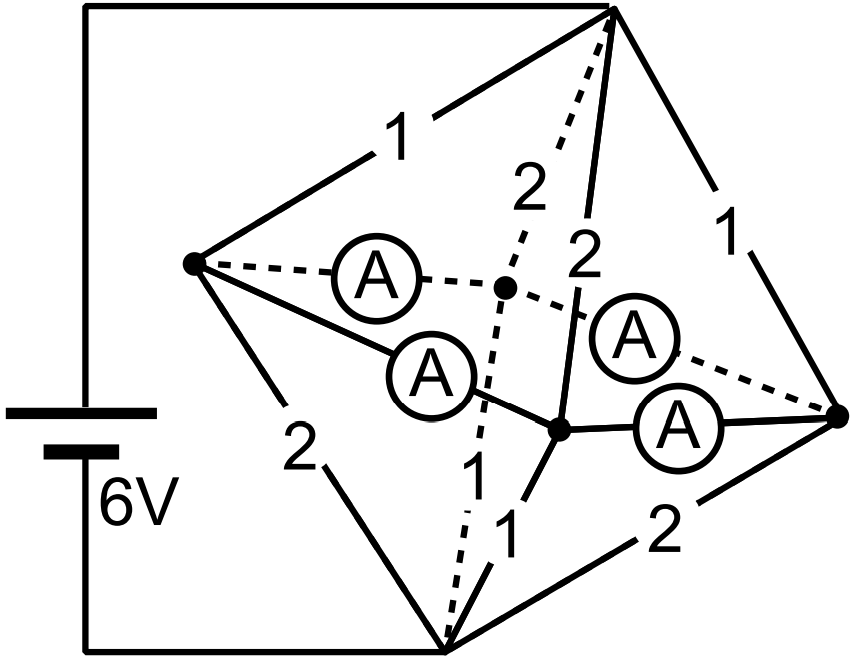
\includegraphics[width=0.5\textwidth]{2016-lahg-08-ampermeeterjoonis}
\end{center}
\fi


\ifEngHint
Since the inner resistance of the ammeters is 0 we can short-circuit them: all the tips where the ammeters lead have equal potentials. Due to symmetry that potential must fall exactly between the potentials of the battery leads, therefore the voltage on each resistor is 3 V.
\fi


\ifEngSolution
Since the inner resistance of the ammeters is zero we can short-circuit them: the potentials on all the tips that the ammeters lead to are equal. Due to symmetry this potential must be exactly between the potentials of the battery’s leads, therefore the voltage 3 V is applied to each resistor. So the current through the 1 ohm resistors is 3 A and the 2 ohm resistors 1.5 A. Due to symmetry this difference of currents is divided equally between two ammeters on each tip, meaning that all the ammeters have the reading 0.75 A.
\fi
}